%
% Complete documentation on the extended LaTeX markup used for Insight
% documentation is available in ``Documenting Insight'', which is part
% of the standard documentation for Insight.  It may be found online
% at:
%
%     http://www.itk.org/

\documentclass{InsightArticle}


%%%%%%%%%%%%%%%%%%%%%%%%%%%%%%%%%%%%%%%%%%%%%%%%%%%%%%%%%%%%%%%%%%
%
%  hyperref should be the last package to be loaded.
%
%%%%%%%%%%%%%%%%%%%%%%%%%%%%%%%%%%%%%%%%%%%%%%%%%%%%%%%%%%%%%%%%%%
\usepackage[dvips,
bookmarks,
bookmarksopen,
backref,
colorlinks,linkcolor={blue},citecolor={blue},urlcolor={blue},
]{hyperref}
% to be able to use options in graphics
\usepackage{graphicx}
% for pseudo code
\usepackage{listings}
% subfigures
%\usepackage{subfigure}


%  This is a template for Papers to the Insight Journal. 
%  It is comparable to a technical report format.

% The title should be descriptive enough for people to be able to find
% the relevant document. 
\title{Histogram-based thresholding - some missing methods}

% 
% NOTE: This is the last number of the "handle" URL that 
% The Insight Journal assigns to your paper as part of the
% submission process. Please replace the number "1338" with
% the actual handle number that you get assigned.
%
\newcommand{\IJhandlerIDnumber}{}

% Increment the release number whenever significant changes are made.
% The author and/or editor can define 'significant' however they like.
\release{0.00}

% At minimum, give your name and an email address.  You can include a
% snail-mail address if you like.
\author{Richard Beare}
\authoraddress{Monash University}

\begin{document}


%
% Add hyperlink to the web location and license of the paper.
% The argument of this command is the handler identifier given
% by the Insight Journal to this paper.
% 
\IJhandlefooter{\IJhandlerIDnumber}{3279}

\maketitle

\ifhtml
\chapter*{Front Matter\label{front}}
\fi


\begin{abstract}
\noindent
% The abstract should be a paragraph or two long, and describe the
% scope of the document.
Using intensity histograms to estimate image thresholds is a long
established practice in image processing and image analysis and a wide
variety of techniques have been developed. Different techniques are
appropriate for different intensity distributions. This article
implements a number of standard techniques not currently available in
ITK.
\end{abstract}

\IJhandlenote{\IJhandlerIDnumber}

\tableofcontents

\section{Introduction}
This contribution includes classes for threshold estimation using the
following methods: Huang\cite{huang1995image},
Intermodes\cite{prewitt1965analysis},
Minimum\cite{prewitt1965analysis}, IsoData\cite{ridler1978picture},
Li\cite{li1993minimum,li1998iterative}, MaxEntropy\cite{kapur1985new},
KittlerIllingworth\cite{kittler1986minimum},
Moments\cite{tsai1985moment}, Yen\cite{yen1995new},
RenyiEntropy\cite{kapur1985new},
Shanbhag\cite{shanbhag1994utilization} and
Triangle\cite{zack1977automatic}.

All classes are largely derived from the AutoThresh
\cite{LandiniImageJ} package for ImageJ. The brief outline below is
taken from the presentation associated with the
HistThresh\cite{HistThreshMatlab} matlab toolbox, which was also a
source of information for the AutoThresh package. The exception is the
triangle method, that was written before discovery of the AutoThresh
packge and before this project got slightly out of hand.

Latest version of this contribution is available via github:
{\tt git clone git://github.com/richardbeare/HistThresh.git}

\section{Thresholding algorithms}
The histogram of the standard cthead image, and the thresholds
estimated by the various methods are shown in Figures \ref{fig:cthead}
and \ref{fig:thresh}
\subsection{Huang}
Huang's fuzzy thresholding using Shannon's entropy function.
\subsection{Intermodes}
Iteratively smooths histogram until only 2 peaks remain. Threshold is
the midpoint of the two peaks. Not good for histograms with very
unequal peaks.
\subsection{Minimum}
Same as Intermodes, except that threshold is the mimimum point between
the peaks, rather than midway. This method is part of the {\em
  itkIntermodeThresholdImageFilter} and is selected using the
{\em UseIntermodeOff} method.
\subsection{IsoData}
Computes average of voxels below initial threshold and above initial
threshold. Threshold is set to the average of the two. Repeat until
the threshold is larger than the composite average.

\subsection{Li}
Li's minimum cross entropy.
\subsection{MaxEntropy}
Choose threshold such that the entropies of distributions above and
below threshold is maximised. One of several entropy-based approaches.

\subsection{KittlerIllingworth}
Similar to the Otsu method. Assumes a Gaussian mixture
model. Minimizes the number of misclassifications between the two
normal distributions with the given means, variances and proportions.
\subsection{Moments}
Choose threshold such that the binary image has the same first three moments as the grey level image.
\subsection{Yen}
Maximum correlation criterion.
\subsection{RenyiEntropy}
Similar to MaxEntropy, but using a different entropy measure.
\subsection{Shanbhag}
Extenstion of the Kapur method.

\subsection{Triangle}
The triangle method constructs a line between the histogram peak and
the farthest end of the histogram. The threshold is the point of
maximum distance between the line and the histogram. This
implementation uses robust (default is 1\% and 99\%) estimation of histogram ends.

\begin{figure}[htbp]
\centering
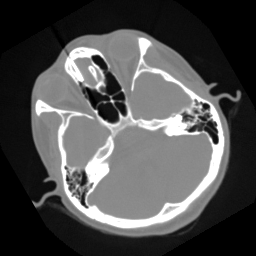
\includegraphics[height=5cm]{cthead1}
\caption{The input image.\label{fig:cthead}}
\end{figure}

\begin{figure}[htbp]
\centering
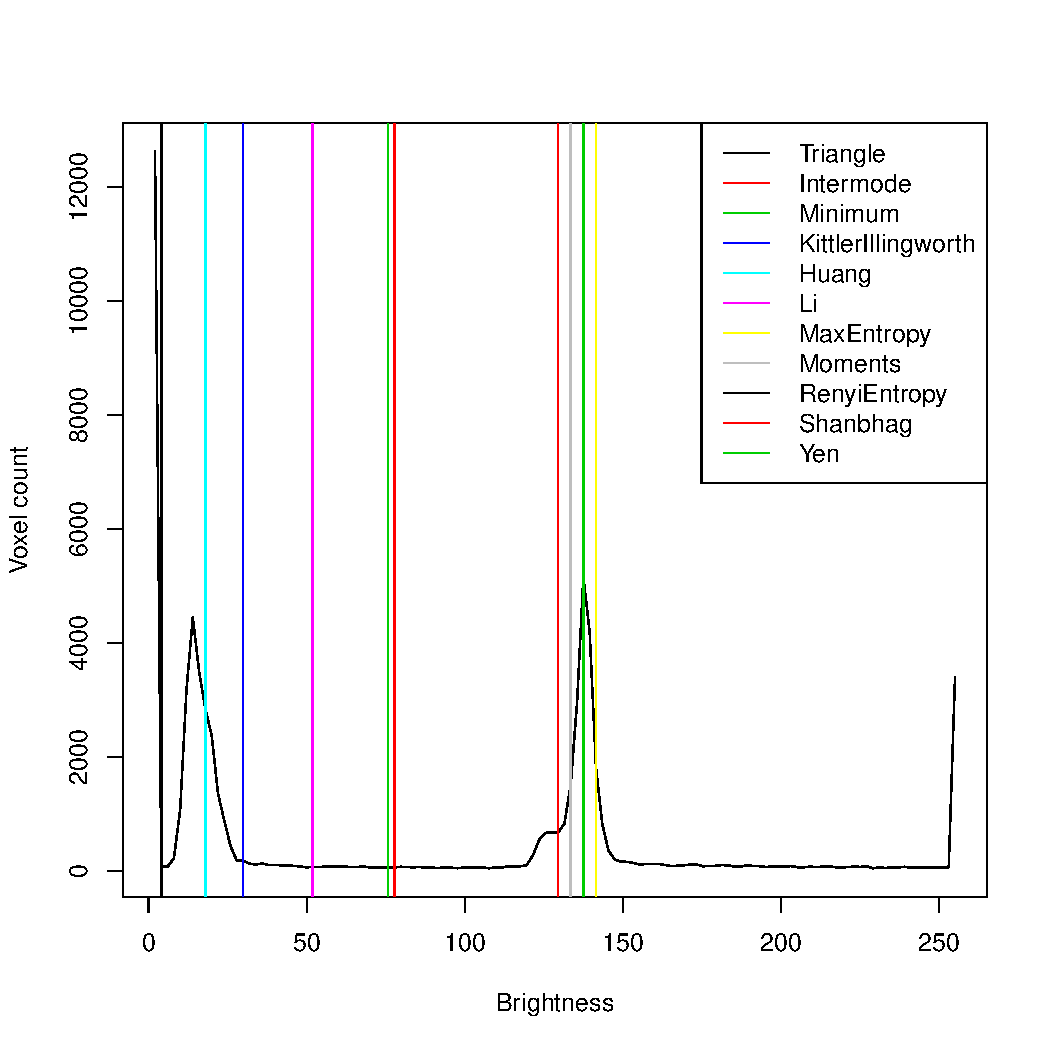
\includegraphics[height=15cm]{hist_results}
\caption{Image histogram and thresholds selected by implemented methods.\label{fig:thresh}}
\end{figure}

\section{Usage}
The new classes are:
\begin{itemize}
\item {\em itkHuangThresholdImageFilter}
\item {\em itkIntermodesThresholdImageFilter}
\item {\em itkIsoDataThresholdImageFilter}
\item {\em itkKittlerIllingworthThresholdImageFilter}
\item {\em itkLiThresholdImageFilter}
\item {\em itkMaxEntropyThresholdImageFilter}
\item {\em itkMomentsThresholdImageFilter}
\item {\em itkRenyiEntropyThresholdImageFilter}
\item {\em itkShanbhagThresholdImageFilter}
\item {\em itkTriangleThresholdImageFilter}
\item {\em itkYenThresholdImageFilter}
\end{itemize}
All classes have methods to set the number of histogram
bins. Intermodes has a method to select the intermodes or minimum
selection option.

Simple test functions are provided for all classes. 



\section{Future improvements}
All classes in this package were based on the existing ITK
implementation of the Otsu method. This class does not make use of the
rich ITK histogram structure, and hence the new classes do not utilize
it either. There is also a moderate amount of repeated code between
the different filter and calculator classes. Future work should look
at refactoring the classes and making better use of the ITK histogram
tools.

More informative examples would also be a great advantage.

\section{Refactoring for ITK 4}
Significant recent work has been carried out for ITK 4. All histogram
calculation methods have been moved to calculator classes - e.g. {\em
  itkYenThresholdCalculator}. Histograms are created using the {\em
  ImageToHistogramImageFilter}, thus utilizing the ITK histogram
facilities. The {\em itkHistogramThresholdingImageFilter} has been
introduced that includes all threshold calculation methods. The method
can be selected via the {\em SetThreshMethod} call.
\begin{verbatim}
filter->SetThreshMethod(FilterType::HUANG);
\end{verbatim}

These additions are available in Gerrit:

\section{Conclusions}
This contribution is a set of standard thresholding methods available
in other packages. The implementation is derived from both the ImageJ
java plugin and the ITK Otsu classes. The classes are being made
available to the user community in a relatively untested and poorly
documented state.  I hope that someone finds them useful. Additional
documentation is welcome.

\appendix



\bibliographystyle{plain}
\bibliography{local}
\nocite{ITKSoftwareGuide}

\end{document}

